\subsection*{Example}
%-------------------------------------------
\begin{frame}{The biological study example}
%-------------------------------------------
\begin{itemize}
    \item Study of the green alga {\it Ostreococcus tauri} response to iron deprivation. 
    \item 16 RNAseq samples in triplicate, single-end of 100bp.
    \item Choice of the 9h point of the long-term adaptative response (s11 and s12 samples):
\end{itemize}
\begin{center}
   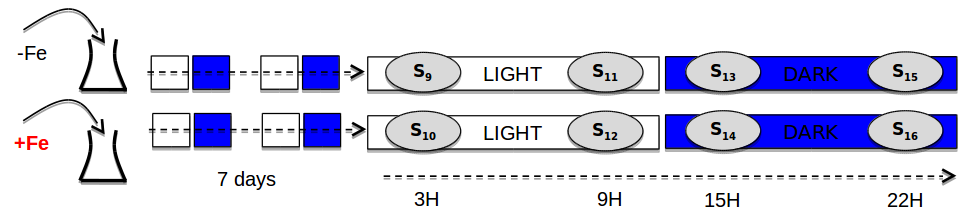
\includegraphics[height=2.5cm]{01_introduction/images/OTauri_Fe_longTerm.png}
\end{center}

\tiny{
Lelandais G, Scheiber I, Paz-Yepes J, Lozano JC, Botebol H, Pilátová J, Žárský V, Léger T, Blaiseau PL, Bowler C, Bouget FY, Camadro JM, Sutak R, Lesuisse E.\\
Ostreococcus tauri is a new model green alga for studying iron metabolism in eukaryotic phytoplankton.\\
\it{BMC Genomics}. 2016 May 3;17:319. doi: 10.1186/s12864-016-2666-6.}
\end{frame}
%-------------------------------------------
\begin{frame}{Reduced RNAseq Data}
%-------------------------------------------
\begin{block}{Genome}
    \begin{itemize}
        \item sequence: GCF\_000214015.3\_version\_140606\_genomic.fna (\url{https://www.ncbi.nlm.nih.gov/assembly/GCF_000214015.3/})
        \item annotation: GCF\_000214015.3\_version\_140606\_genomic.gff
        \item $\Rightarrow$ 13.0328 Mb, 20 chromosomes, mitochondria, $\&$ chloroplast
    \end{itemize}
\end{block}
\begin{block}{RNAseq samples}
    \begin{itemize}
      \item Project: \href{https://www.ebi.ac.uk/ena/browser/view/PRJNA304086}{PRJNA304086}
      \item Selection samples 11 and 12: SRR3099585-87, SRR3105697-99 (fastq.gz ${\sim}$360M each x 6 files)
      \item Reads selection to reduce data volume for the course (mapped on the smalest chromosome, chr18, NC\_014443.2 + 100000 first) $\Rightarrow$ *$\_$chr18.fastq.gz ${\sim}$19M each (\small{\url{https://zenodo.org/record/3997237}})
      \item Counts table, complete RNAseq: \small{\url{https://zenodo.org/record/4008452}}
    \end{itemize}
\end{block}
\end{frame}
%-------------------------------------------
\begin{frame}[containsverbatim]
\frametitle{Data}
%-------------------------------------------
\begin{exampleblock}{Access in the IFB ressources}
\begin{lstlisting}
/shared/projects/fair_training2020/Data/
\end{lstlisting}
\end{exampleblock}
\begin{exampleblock}{Or raw download in a local "Data" directory}
\begin{lstlisting}
mkdir Data ; cd Data
wget https://ftp.ncbi.nlm.nih.gov/genomes/all/GCF/000/214/015/GCF_000214015.3_version_140606/GCF_000214015.3_version_140606_genomic.fna.gz
wget https://ftp.ncbi.nlm.nih.gov/genomes/all/GCF/000/214/015/GCF_000214015.3_version_140606/GCF_000214015.3_version_140606_genomic.gff.gz
wget https://zenodo.org/record/3997237/files/FAIR_Bioinfo_data.tar.gz
wget https://zenodo.org/record/3997137/files/counts.txt
cd ..
\end{lstlisting}
\end{exampleblock}
\end{frame}
%-------------------------------------------
\begin{frame}[label=RNAseqWF_diapo]{RNAseq analysis}
%-------------------------------------------
\begin{block}{Analysis workflow}
    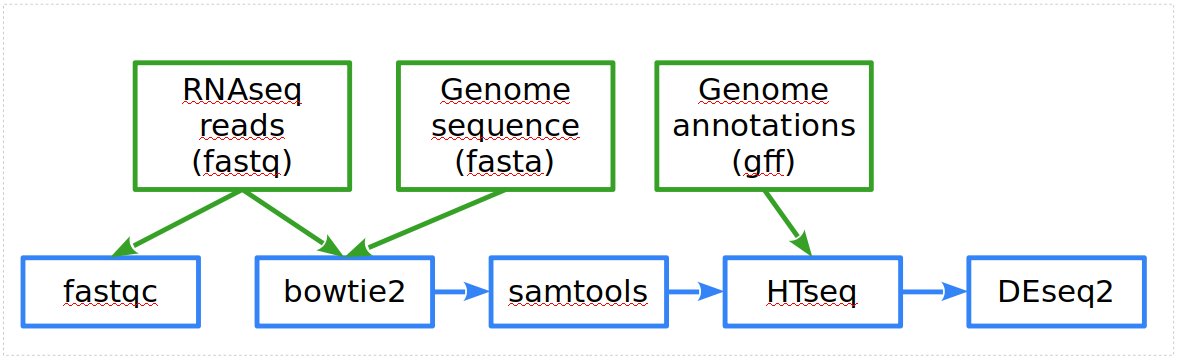
\includegraphics[width=12cm]{01_introduction/images/FAIR_RNAseq_WF.png}\\
green=input, blue=tool
\end{block}
\footnotesize{
\begin{description}
    \item[fastqc] control quality of the input reads
    \item[bowtie2] reads mapping on the genome sequence
    \item[samtools] mapped reads selection $\&$ formatting
    \item[HTseq] count table of mapped reads on genes (annotations)
    \item[DEseq2] statistical analysis: genes list having differential expression
\end{description}
}
\end{frame}
%-------------------------------------------
\begin{frame}[label=RNAseqWF2skill_diapo]{2 bioinformatician skills}
%-------------------------------------------
\begin{block}{Analysis workflow}
    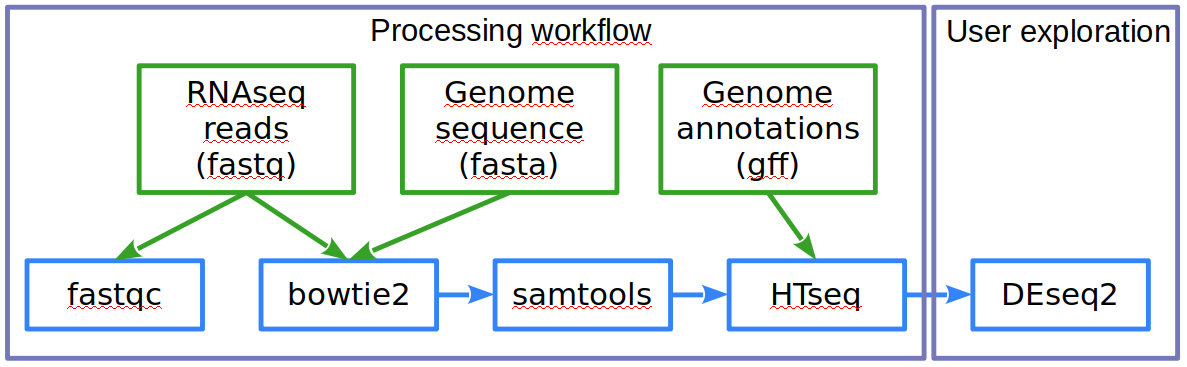
\includegraphics[width=12cm]{01_introduction/images/FAIR_RNAseq_WF_2skills.png}\\
green=input, blue=tool, violet=skill
\end{block}
\begin{block}{Reproducibility}
\begin{description}
    \item[Processing workflow] automatization, scripting
    \item[User exploration] report choices (or import choices for further analysis) 
\end{description}
\end{block}
\end{frame}